\documentclass{article}
\usepackage[utf8]{inputenc}
\usepackage{url}
\usepackage{fancyhdr}
\usepackage[ddmmyyyy]{datetime}

\usepackage{amsfonts}

\usepackage[top=2cm, bottom=2cm, left=1.5cm, right=1.5cm]{geometry}

\usepackage{natbib}
\usepackage{graphicx}

\usepackage{xcolor}
\usepackage{listings}
\lstset{basicstyle=\ttfamily,
  showstringspaces=false,
  commentstyle=\color{red},
  keywordstyle=\color{blue}
}
\lstdefinelanguage{json}{
    string=[s]{"}{"},
    stringstyle=\color{red},
    comment=[l]{:},
    commentstyle=\color{black},
}
\lstset{escapeinside={<@}{@>}}

\newcommand{\version}{V0.3}

 
\pagestyle{fancy}
\fancyhf{}
\rhead{\today}
\chead{\version}
\lhead{\url{t.fontana@net2action.com}}
\rfoot{Page \thepage}

\title{Analisi e Descrizione Iniziali del Plugin \\ \textbf{CheckTime \version}}
\author{Tommaso Fontana}


\begin{document}

\maketitle

\begin{abstract}
Descrizione iniziale del plugin che analizzando i valori di utilizzo del disco di una macchina di un dato periodo di tempo \(\Delta t\) stima quanto tempo rimane prima della saturazione di un risorsa e genera warning nel caso il tempo sia inferiore a certe threshold. L'utilizzo principale pensato per lo script e' monitorare lo stato dei dischi ma lo script e' abbastanza generale da poter trattare anche altri casi (e.g. CPU/RAM) purche' sia definito il valore attuale e quello massimo.
\end{abstract}

\clearpage

\part*{Descrizione del problema}
Attualmente le threshold di warning e critical per i dischi dei server sono espresse in bytes.
\\\\
Questo ovviamente risulta poco utile nel caso di server maturi il cui utilizzo del disco cambia poco nel tempo.
\\\\
Ad esempio un server il cui unico scopo e' agire da firewall avra' raramente bisogno di occupare ulteriore spazio su disco, quindi anche nel caso avesse libero solo 1Gb di spazio sul disco questo potrebbe funzionare indisturbato per anni.
\\\\
L'esempio diametralmente opposto e' un server che ospita un Database il quale potrebbe occupare quel Gigabyte in una manciata di ore.
\\\\
Quindi chiaramente lo spazio rimanente non e' una metrica affidabile ed utile in generale.
\\\\
La soluzione proposta da questo plugin e' quella di stimare quanto tempo rimane alla saturazione del disco (raggiungimento del 100\% di utilizzo) analizzando lo storico dati dell'ultimo periodo.
\\\\
Il valore aggiunto di potere, a questo punto, avere le threshold espresse in una qualche unita' di tempo e' la possibilita' di essere avvisati tempestivamente.
\\\\
Ad esempio che supponendo che per ordinare un disco aggiuntivo ed installarlo servano al massimo 5 giorni si poter impostare la threshold critica a 6 giorni in modo da essere avvisati un giorno prima del tempo minimo per garantire la continuità del servizio.
\\\\
E si potrebbe impostare la threshold di warning ad esempio ad 1 mese in modo da poter ordinare i dischi in anticipo in modo da essere preparati al' eventuale saturazione del disco.
\\\\
Inoltre cio' evita falsi allarmi, nel caso del firewall enunciato prima l'utente avrebbe un messaggi di warning / critical anche se potrebbero volerci anni a saturare il disco effettivamente.
\\\\
Infine permette di avere dati oggettivi e quantificabili su cui poter ragionare invece che grafici che lasciano spazio all'interpretazione.
Questo permette un'organizzazione piu' precisa ed oggettiva.
\\\\
Il caso dei dischi e' solo uno dei vari casi in cui avere una metrica espressa in tempo risulta utile rispetto ad averla espressa nella sua unita'.
\\\\
Un altro caso potrebbe essere l'utilizzo di RAM / CPU di un server.\\
Con il passare del tempo, ci si aspetta che il numero di utenti cresca.\\
Con piu' utenti attivi il servizio richiedera' piu' risorse, quindi con questo script potremmo prevedere quando servira' fare scaling (verticale o orizzontale) dei server che gestiscono il serivzio.
\\
Il principale vantaggio e' che questo permette di creare una stima di un piano di investimento nel tempo per adeguare l'hardware alla crescita del servizio.


\clearpage

\part*{Descrizione Implementazione del Plugin}
\textbf{Premessa}: Come verra' descirtto piu' avanti avremo bisogno di due frontend, uno per windows ed uno per linux. Questi sono \textit{checktimewin, checktimelinux} ma in generale quando non e' necessario specificare il sistema operativo perche' si parla di feature comuni verra' scritto solamente \textit{checktime} omettendo l'OS per quanto l'eseguibile \textit{checktime} non esiste.
\section*{Descrizione Installazione e Configurazione}
Lo script non avra' bisogno di alcuna dipendenza poiche' autocontenuto nella cartella.\\
La procedura di installazione sara' soltanto la copia della cartella sul sistema e la creazione del file di cron-job che avra' sintassi simile a:

\begin{lstlisting}[language=Bash]
*/5 * * * * <@\textcolor{red}{/var/checktime/checktime}@> -H "rt-sccm01-p1.idolrt.regione.toscana.it"
    -s "Diskspace" -m "Win" -n "1d" -w "4w" -c "1w"
\end{lstlisting}

\subsection*{Aggiunta dello script al PATH}
Si puo' creare un link simbolico:
\begin{lstlisting}[language=Bash]
$ sudo ln -s /var/checktime/checktimewin   /bin/checktimewin
$ sudo ln -s /var/checktime/checktimelinux /bin/checktimelinux
\end{lstlisting}

cosi che in tutto il sistema si possa chiamare \textit{checktime} come qualsiasi altro commando nel \textit{PATH}.
\\\\
Cio' permette di avere il file di cron che non deve avere hardcodato il path di installazione di \textit{checktime}:

\begin{lstlisting}[language=Bash]
*/5 * * * * <@\textcolor{red}{checktime}@> -H "rt-sccm01-p1.idolrt.regione.toscana.it"
    -s "Diskspace" -m "Win" -n "1d" -w "4w" -c "1w"
\end{lstlisting}

\subsection*{Configurazione accesso DB}

Nella cartella ci sara' un file \textit{db\_settings.json} che conterra' le settings per connettersi al DB che avra' sintassi simile a:

\begin{lstlisting}[language=json]
{
    "database": "icinga2",
    "host": "127.0.0.1",
    "port": 8086,
    "username": "root",
    "password": "",
    "ssl": true,
    "verify_ssl": true,
    "timeout": 60,
    "retries": 3,
    "use_udp": false,
    "udp_port": 4444,
    "proxies": {},
    "path": ""
  }
\end{lstlisting}

\section*{Descrizione Aggiornamento}
Il plugin verrà sviluppato in un repository quindi una volta rilasciata la nuova versione bastera' eseguire il seguente comando (o comunque una sua versione alternativa) nella cartella di installazione per aggiornare:
\begin{lstlisting}[language=Bash]
$ git pull
\end{lstlisting}

\clearpage

\section*{Descrizione Utilizzo}

\subsection*{Input}
Poiche' gli schema dei db sono diversi a seconda del fatto che il sistema sia \textcolor{blue}{Windows} o \textcolor{red}{Linux} avremo bisogno di due "frontend" per poter passare i dati allo script core.\\
Rispettivamente gli eseguibili \textit{checktimewin} e \textit{checktimelinux}.\\
Quando possibile, per essere il piu' generali possibili verra' scritto \textit{checktime} omettendo il sistema operativo specifico per quanto l'eseguibile \textit{checktime} non esiste.
\\
\\
Nello specifico gli schema dei measurements per i due sistemi sono:

\begin{lstlisting}[]
<@\textcolor{blue}{Windows}@>:
time, hostname, matric, service, warn, crit, max, unit, value
<@\textcolor{red}{Linux}@>:
time, device, free, fstype, host, inodes_free, inodes_total, 
    mode, path, total, used_percent
\end{lstlisting}

\subsubsection*{\textcolor{blue}{Windows} frontend}
\begin{lstlisting}[]
$ ./checktimewin -h
usage: main_win.py [-h] -M MEASUREMENT -n WINDOW -w WARNING_THRESHOLD -c
                   CRITICAL_THRESHOLD [-v {0,1}]<@\textcolor{blue}{ -H HOST -s SERVICE}@>
                   <@\textcolor{blue}{[-m METRIC] [-e EXCLUDE]}@>

optional arguments:
  -h, --help            show this help message and exit

query settings (required):
  -M MEASUREMENT, --measurement MEASUREMENT
                        measurement where the data will be queried.

thresholds settings:
  -n WINDOW, --window WINDOW
                        the range of time to consider in the analysis.
  -w WARNING_THRESHOLD, --warning-threshold WARNING_THRESHOLD
                        the time that if the predicted time is lower the
                        script will exit(1).
  -c CRITICAL_THRESHOLD, --critical-threshold CRITICAL_THRESHOLD
                        the time that if the predicted time is lower the
                        script will exit(2).

verbosity settings (optional):
  -v {0,1}, --verbosity {0,1}
                        set the logging verbosity, 0 == ERROR, 1 == DEBUG, it
                        defaults to ERROR.

<@\textcolor{blue}{os dependant settings (required) Windows:}@>
  <@\textcolor{blue}{-H HOST, --host HOST  host which disks will be checked.}@>
  <@\textcolor{blue}{-s SERVICE, --service SERVICE}@>
                        <@\textcolor{blue}{service to be checked.}@>

<@\textcolor{blue}{os dependant settings (optional) Windows:}@>
  <@\textcolor{blue}{-m METRIC, --metric METRIC}@>
                        <@\textcolor{blue}{metric to be checked.}@>
  <@\textcolor{blue}{-e EXCLUDE, --exclude EXCLUDE}@>
                        <@\textcolor{blue}{metric to be excluded from the analysis.}@>

\end{lstlisting}
\clearpage
\subsubsection*{Esempio di utilizzo}

\begin{lstlisting}[language=Bash]
$ checktime  <@\textcolor{gray}{-M "disk"}@>  <@\textcolor{blue}{-H "rt-sccm01-p1.idolrt.regione.toscana.it"}@> 
    <@\textcolor{green!10!orange!90!}{-s "Diskspace"}@> <@\textcolor{red}{-m "C:/"}@> <@\textcolor{green!20!blue!80!}{-n "1d"}@> <@\textcolor{black!30!green!70!}{-w "4w"}@> <@\textcolor{black!30!magenta!70!}{-c "1w"}@>
\end{lstlisting}

Il quale controllera' dal \textcolor{gray}{measurement \textit{disk}} per \textcolor{blue}{l'host \textit{"rt-sccm01-p1.idolrt.regione.toscana.it"}}, \textcolor{green!10!orange!90!}{il servizio \textit{"Diskspace"}} per  \textcolor{red}{la metrica \textit{"C:/"}} utilizzando \textcolor{green!20!blue!80!}{i dati dell'ultimo giorno} e generera' un \textcolor{black!30!green!70!}{warning se il tempo previsto e'  inferiore a 4 settimane} \textcolor{black!30!magenta!70!}{ed un critical error nel caso sia inferiore ad una settimana}.
\\\\

\subsubsection*{\textcolor{red}{Linux} frontend}
Lo script dovra' sapere su quale Host, Servizio e opzionalemnte Metrica fare la analisi.
Questi dati dovranno essere passati allo script tramite riga di comando nella seguente sintassi:
\begin{lstlisting}[]
$ ./checktimelinux -h
usage: main_linux.py [-h] -M MEASUREMENT -n WINDOW -w WARNING_THRESHOLD -c
                     CRITICAL_THRESHOLD [-v {0,1}] <@\textcolor{red}{-H HOST -d DEVICE}@>
                     <@\textcolor{red}{[-p PATH] [-e EXCLUDE]}@>
optional arguments:
  -h, --help            show this help message and exit

query settings (required):
  -M MEASUREMENT, --measurement MEASUREMENT
                        measurement where the data will be queried.

thresholds settings:
  -n WINDOW, --window WINDOW
                        the range of time to consider in the analysis.
  -w WARNING_THRESHOLD, --warning-threshold WARNING_THRESHOLD
                        the time that if the predicted time is lower the
                        script will exit(1).
  -c CRITICAL_THRESHOLD, --critical-threshold CRITICAL_THRESHOLD
                        the time that if the predicted time is lower the
                        script will exit(2).

verbosity settings (optional):
  -v {0,1}, --verbosity {0,1}
                        set the logging verbosity, 0 == ERROR, 1 == DEBUG, it
                        defaults to ERROR.

<@\textcolor{red}{os dependant settings (required) Linux:}@>
  <@\textcolor{red}{-H HOST, --host HOST  host which disks will be checked.}@>
  <@\textcolor{red}{-d DEVICE, --device DEVICE}@>
                        <@\textcolor{red}{service to be checked.}@>

<@\textcolor{red}{os dependant settings (optional) Linux:}@>
  <@\textcolor{red}{-p PATH, --path PATH  metric to be checked.}@>
  <@\textcolor{red}{-e EXCLUDE, --exclude EXCLUDE}@>
                        <@\textcolor{red}{path to be excluded from the analysis.}@>

\end{lstlisting}

\clearpage
\section*{Cornercases}
Poiche' si cerca di mantenere il comportamento dei frontend il piu' omogeneo possibile varra' la equivalenza tra:

\begin{lstlisting}[language=Bash]
-d DEVICE <-> -s SERVICE
-p PATH   <-> -m METRIC
\end{lstlisting}
e gli \textit{-e} funzioneranno esattamente nello stesso modo pero' si riferiranno a \textit{PATH} o a \textit{METRIC} a seconda del frontend.

La gerarchia dei field per i due sistemi quindi sara':
\begin{lstlisting}[language=Bash]
<@\textcolor{blue}{Windows}@>:
Measurement > Host > Service > Metric
<@\textcolor{red}{Linux}@>:
Measurement > Host > Device > Path
\end{lstlisting}
Per cercare di rendere la trattazione il piu' omogenea e predittbile possibile.

\subsubsection*{Cornercase: Cosa succede se uno o piu' parametri richiesti non sono passati}
Se un parametro rischiesto o piu' non viene passato lo script uscira' con \textbf{exit(1)} ed elenchera' quali parametri mancano sulla \textbf{stderr}.
\\
e.g. se lo script viene chiamato senza parametri:
\begin{lstlisting}[language=Bash]
$ checktime
usage: checktime [-h] -M MEASUREMENT -H HOST -s SERVICE [-m METRIC] [-e EXCLUDE]
               -n WINDOW -w WARNING_THRESHOLD -c CRITICAL_THRESHOLD [-v {0,1}]
checktime: error: the following arguments are required:
-M/--measurement, -H/--host, -s/--service, -n/--window,
-w/--warning-threshold, -c/--critical-threshold
\end{lstlisting}

\subsubsection*{Cornercase: Cosa succede se uno o piu' parametri non esisto sul DB}
Se uno o piu' parametri non esistono sul DB (eccetto le metriche) allora lo script uscira' con \textbf{exit(1)} e descrivera' quali parametri non sono stati trovati sulla \textbf{stderr}.
\\
Lo script si ferma al primo parametro non trovato con ordine di priorita':
\begin{lstlisting}[language=Bash]
<@\textcolor{blue}{Windows}@>:
Measurement > Host > Service > Metric
<@\textcolor{red}{Linux}@>:
Measurement > Host > Device > Path
\end{lstlisting}
Il caso in cui una metrica non esiste viene affrontato piu' avanti.\\
e.g. se si sbaglia a scrivere \textit{"disk"} e si scrive \textit{"disck"}:
\begin{lstlisting}[language=Bash]
$ checktime -M "disck" -H "rt-sccm01-p1.idolrt.regione.toscana.it" 
    -s "Diskspace" -n "1d" -w "4w" -c "1w"
<@\textcolor{red}{error: measurement "disck" not found.}@>
\end{lstlisting}

e.g. se si sbaglia a scrivere l'host:
\begin{lstlisting}[language=Bash]
$ checktime -M "disk" -H "rt-sccm01-p1.idolrt.regione.toscana.com" 
    -s "Diskspace" -n "1d" -w "4w" -c "1w"
<@\textcolor{red}{error: host "rt-sccm01-p1.idolrt.regione.toscana.com" not found.}@>
\end{lstlisting}

e.g. se si sbaglia a scrivere il service:
\begin{lstlisting}[language=Bash]
$ checktime -M "disk" -H "rt-sccm01-p1.idolrt.regione.toscana.it" 
    -s "diskspace" -n "1d" -w "4w" -c "1w"
<@\textcolor{red}{error: service "diskspace" not found.}@>
\end{lstlisting}

\clearpage
\subsection*{Scelta delle metriche / path}
\subsubsection*{Selezione delle metriche / path}
Se allo script non viene passato nessun parametro \textit{-m/-p} allora lo script selezionera' di default tutte le metriche / path presenti sul DB.

e.g.:
\begin{lstlisting}[language=Bash]
$ checktime -M "disk" -H "rt-sccm01-p1.idolrt.regione.toscana.it" 
    -s "Diskspace" -n "1d" -w "4w" -c "1w"
/ 1y3d4s
/produzione 3w
/var 5d
/mnt 6w
/tmp 1s
\end{lstlisting}

Se invece vogliamo analizzare solo un subset ti metriche queste dovranno essere passate ciascuna con un parametro \textit{-m}.\\

e.g.:
\begin{lstlisting}[language=Bash]
$ checktime -M "disk" -H "rt-sccm01-p1.idolrt.regione.toscana.it" 
    -s "Diskspace" <@\textcolor{red}{-p "/" -p "/produzione"}@> -n "1d" -w "4w" -c "1w"
/ 1y3d4s
/produzione 3w
\end{lstlisting}

\subsubsection*{Filtraggio delle metriche / path}
Se si vuole escludere qualche metrica / path dalla analisi basta passarla al parametro \textit{-e}.\\

e.g. analizzare tutto ma escludere \textit{/tmp, /var, /mnt}: 
\begin{lstlisting}[language=Bash]
$ checktime -M "disk" -H "rt-sccm01-p1.idolrt.regione.toscana.it" 
    -s "Diskspace"  <@\textcolor{red}{-e "/tmp" -e "/var" -e "/mnt"}@> -n "1d" -w "4w" -c "1w"
/home 1d2s
/produzione 1y3d
\end{lstlisting}

\subsubsection*{Cornercase: presenza di entrambi \textit{-m, -e}}

I parametri \textit{-m/p} ed \textit{-e} sono combinabili.

e.g. questo script analizzera' solo \textit{/tmp}: 
\begin{lstlisting}[language=Bash]
$ checktime -M "disk" -H "rt-sccm01-p1.idolrt.regione.toscana.it" 
    -s "Diskspace"  <@\textcolor{red}{-p "/tmp" -p "/var" -e "/var"}@> -n "1d" -w "4w" -c "1w"
/tmp 1y2w4s
\end{lstlisting}

Questa scelta e' stata fatta per mantenere consistenza nel utilizzo dei parametri e perche' potrebbe essere utile in caso di debug di poter disabilitare una metrica temporaneamente senza il rischio di dimenticare quale fosse.

\subsubsection*{Cornercase: \textit{-e} di una metrica non esistente}
Nel caso eseguissimo un \textit{-e} su una metrica non presente sul DB questa verrà ignorata e non genererà alcun tipo di errore o warning.
\\
e.g. questo script non genera' errori o warning a causa della non esistenza di \textit{C:/} o \textit{/tmp}: 
\begin{lstlisting}[language=Bash]
$ checktime -M "disk" -H "rt-sccm01-p1.idolrt.regione.toscana.it" 
    -s "Diskspace"  <@\textcolor{red}{-e "C:/" -e "/tmp"}@> -n "1d" -w "4w" -c "1w"
\end{lstlisting}


\subsubsection*{Cornercase: \textit{-m/p} di una metrica / path non esistente}
Nel caso eseguissimo un \textit{-m/p} su una metrica / path non presente sul DB questa verrà ignorata nella analisi ma ritornerà uno stato di un warning (\textbf{exit(1)}) e vera' scritto un messaggio di warning sulla \textbf{stderr}.\\
(Nel caso lo script dovesse ritornare \textbf{exit(2)} a causa di un valore fuori threshold allora lo script darà priorità alla \textbf{exit(2)} rispetto al \textbf{exit(1)})
\\
e.g. questo script genera' un warning a causa della non esistenza di \textit{C:/} o \textit{/tmp}: 
\begin{lstlisting}[language=Bash]
$ checktime -M "disk" -H "rt-sccm01-p1.idolrt.regione.toscana.it" 
    -s "Diskspace"  <@\textcolor{red}{-m "C:/" -m "/tmp"}@> -n "1d" -w "4w" -c "1w"
warning: Not found the metric "C:/"
/tmp 1w2d3m
\end{lstlisting}



\clearpage

\subsection{Output}
Nel caso lo script sia andato su una singola metrica l'output scritto sulla \textbf{stdout} sara' simile a:
\begin{lstlisting}[language=Bash]
$ checktime -M "disk" -H "rt-sccm01-p1.idolrt.regione.toscana.it" 
    -s "Diskspace" -m "C:/" -n "1d" -w "4w" -c "1w"
C:/ 1w2d3h
\end{lstlisting}
Nel caso vada su mutiple metriche l'output sara' simile a;

\begin{lstlisting}[language=Bash]
$ checktime -M "disk" -H "rt-sccm01-p1.idolrt.regione.toscana.it" 
    -s "Diskspace" -n "1d" -w "4w" -c "1w"
C:/ 1w2d3h
D:/ 1y3d
E:/ 1m2s
F:/ 2y2w
\end{lstlisting}

In generale seguira' il linguaggio regolare:

\begin{lstlisting}[language=Bash]
(<Nome Metrica> <Tempo Rimasto>\n)+
\end{lstlisting}

Se il tempo rimasto di qualunque metrica sia inferiore al livello di warning lo script avra' exit code 1.

Nel caso qualunque metrica sia inferiore al livello di Critical lo script avra' exit code 2 altrimenti sara' 0.

\subsection*{Caso di tempo infinito}
Nel caso che un disco abbia spazio utlizzato costante o decrescente l'output sara' del simile a:

\begin{lstlisting}[language=Bash]
$ checktime -M "disk" -H "rt-sccm01-p1.idolrt.regione.toscana.it" 
    -s "Diskspace" -n "1d" -w "4w" -c "1w"
C:/  <@\textcolor{red}{inf}@>
D:/ 1y3d
E:/  <@\textcolor{red}{inf}@>
F:/ 2y2w
\end{lstlisting}

\subsection*{Formato del tempo}
La sintassi del tempo dovra' seguire la seguente espressione regolare:

\begin{lstlisting}[]
(inf|(\d+y)?(\d+w)?(\d+d)?(\d+h)?(\d+m)?(\d+s)?) 
\end{lstlisting}

dove la stringa vuota sara' interpretata come 0 secondi.
\\
di seguito esempi di tempo espressi in questa forma, uno per riga:

\begin{lstlisting}[language=Bash]
inf
1y
2000s
1y1w1d1h1m1s
1y10w100d1000h10000m100000s
1y3s
\end{lstlisting}


\clearpage

\section*{Descrizione Cartella}
La cartella dello script avra' la seguente struttura:
\begin{lstlisting}[language=Bash]
drwxr-xr-x 5 user user 4,0K 29 giu 14.25 check_time_venv
drwxr-xr-x 4 user user 4,0K 29 giu 14.21 doc
drwxr-xr-x 3 user user 4,0K  2 lug 23.01 src
drwxr-xr-x 2 user user 4,0K 29 giu 13.51 tests
-rw-r--r-- 1 user user  281 29 giu 13.33 db_settings.json
-rw-r--r-- 1 user user  18K 29 giu 14.22 license
-rw-r--r-- 1 user user   95 29 giu 14.24 README.rst
-rwxr-xr-x 1 user user  102 29 giu 16.26 checktimewin
-rwxr-xr-x 1 user user  103 29 giu 16.27 checktimelinux
\end{lstlisting}

Legenda:
\begin{itemize}
    \item \textbf{check\_time\_venv} E' la cartella del virtual environment di python 3 gia' configurato.
    \item \textbf{doc} La cartella contenete la documentazione e gli esempi di utilizzo dello script.
    \item \textbf{src} La cartella con i sorgenti python dello script.
    \item \textbf{tests} La cartella conetenente i test da poter eseguire post installazione per poter testare che lo script funzioni correttamente.
    \item \textbf{db\_settings.json} E' il file di configurazione per configurare come connettersi al DB.
    \item \textbf{license} La licenza GPL2 dello script.
    \item \textbf{README.rst} File di intro della repo e tutorial veloce su come installare, aggiornare ed utilizzare lo script.
    \item \textbf{checktimelinux} E' l'eseguibile per Linux.
    \item \textbf{checktimewin} E' l'eseguibile per Windows.
\end{itemize}

\clearpage
\part*{Descrizione del metodo di predizione}

\subsection{Descrizione del problema}
Data una serie di valori \(p_i = (t_i, u_i)\) su un intervallo di tempo \(\Delta t\) dove \(u \in [0, 1] \subset \mathbb{R}\) e' l'utilizzo percentuale del  disco e \(t \in \mathbb{N}\) e' il timestamp  della misurazione di \(u\) vogliamo sapere il tempo rimanente \(\Delta t_r\) al quale ci aspettiamo il raggiungimento massimo ( 100\% ) del disco. 

\subsection{Soluzione proposta}
Per semplicità inizialmente la strategia e' quella di supporre una relazione lineare tra uso del disco (\(u\)) e il tempo (\(t\)):
\[u = m t + q\]
per ottenere i due parametri \(m, q \in \mathbb{R}\) ci sono diverse metodologie spiegate dopo.
\\
Una volta ottenuti i parametri \(m, q\) basta invertire l'equazione:
\[u = m t + q \quad \Rightarrow \quad t = \frac{u - q}{m}\]

quindi basta sostituire ad \(u\) l'utilizzo che per cui vogliamo stimare il tempo, in questo caso il 100\% quindi :

\[t_r = \frac{1 - q}{m}\]

in fine per ottenere il tempo rimanente al istante \(t_{now}\)  basta fare:
\[\Delta t_r = t_r - t_{now}\]

\subsection{Soluzione proposta aggiuntiva nel caso di dati molto rumorosi}
Nel caso i dati abbiano molte periodicita' o rumore si potrebbe pensare di eseguire prima di tutto uno smoothing dei dati con una moving window o con un kernel gaussiano.
\\
Poi si potrebbe usare il metodo di \textit{Holt Winter} quindi un \textit{Double} o \textit{Triple Exponential Smoothing} per estrarre trend e periodicita' (questo metodo e' intensivo computazionalmente quindi conviene usarlo solo se strettamente necessario).
\\
Alternativamente al metodo di \textit{Holt Winter}  si potrebbe eseguire una \textit{Trasformata Discreta di Fourier} della differenza tra i valori e il loro trend per identificare le componenti principali ed ad esempio tenere le piu' grandi per predirre i fenomeni  periodici principali.
\\
Questo permetterebbe anche al utente nel caso di avere degli insights sul proprio sistema.

\subsection{Metodi di regressione}
Per stimare la retta che approssima i dati ci sono vari modi, spiegati brevemente qui di seguito in ordine di complessità ed utilità.

Riassunti:
\begin{itemize}
    \item Regressione dei minimi quadrati: Il metodo standard.
    \item RANSAC: Cerca di distinguere i valori dal rumore.
    \item Regressione Bayesiana: Possiamo suggerire al metodo come ci aspettiamo i risultati e sopratutto \textbf{possiamo stimare quanto e' probabile che tra un certo quantitativo di tempo il disco sara' pieno.}
\end{itemize}

\clearpage

\subsubsection{Regressione minimi quadrati}
E' il metodo piu' facile e veloce.\\
Definiamo una funzione che calcola l'errore in funzione dei due paramatri cercati \(m, q\).
\[E(m, q) = \sum_{i = 0}^N \left[u_i - (m t_i + q)\right]^2\]
E vogliamo i parametri che minimizzano l'errore quindi basta imporne il gradiente a zero.

\[\nabla E(m, q) = 0\]

Il che implica che:

\[\frac{\partial E(m, q)}{\partial q} = 2\sum_{i = 0}^N \left[u_i - (m t_i + q)\right] = 0 \rightarrow  \sum_{i = 0}^N u_i - m \sum_{i = 0}^N t_i + q N = 0\]
\[\frac{\partial E(m, q)}{\partial m} = 2\sum_{i = 0}^N \left[u_i - (m t_i + q)\right] \left[u_i\right] = 0 \rightarrow \sum_{i = 0}^N u_i^2 - m \sum_{i = 0}^N t_i u_i + q\sum_{i = 0}^N u_i =  0\]

Le quali formano un sistema lineare di equazioni nelle due incognite \(m, q\) che una volta risolto si ottengono gli stimatori:

\[m = \frac{\sum_{i = 0}^N \left[t_i - \hat{t}\right]\left[u_i - \hat{u}\right]}{\sum_{i = 0}^N \left[t_i - \hat{t}\right]^2}\]

\[q = \hat{u} - m \hat{t} \]

dove \(\hat{t}, \hat{u}\) sono rispettivamente i valori medi di tempo ed utilizzo nella finestra temporale considerata.


\subsubsection{RANSAC (RANdom SAmple Consensus)}

E' un metodo robusto per fare fitting di dati anche in presenza di outliers quindi rumore.
\\\\
 È un algoritmo non deterministico nel senso che produce un risultato corretto solo con una data probabilità, che aumenta al crescere delle iterazioni consentite.\\\\
 L'assunzione di base per il funzionamento è che i dati siano costituiti da dei dati giusti e da dei dati di rumore.\\\\
 Un esempio di applicazione in cui i punti blu sono ritenuti dati e quelli rossi vengono classificati come rumore:
\begin{center}
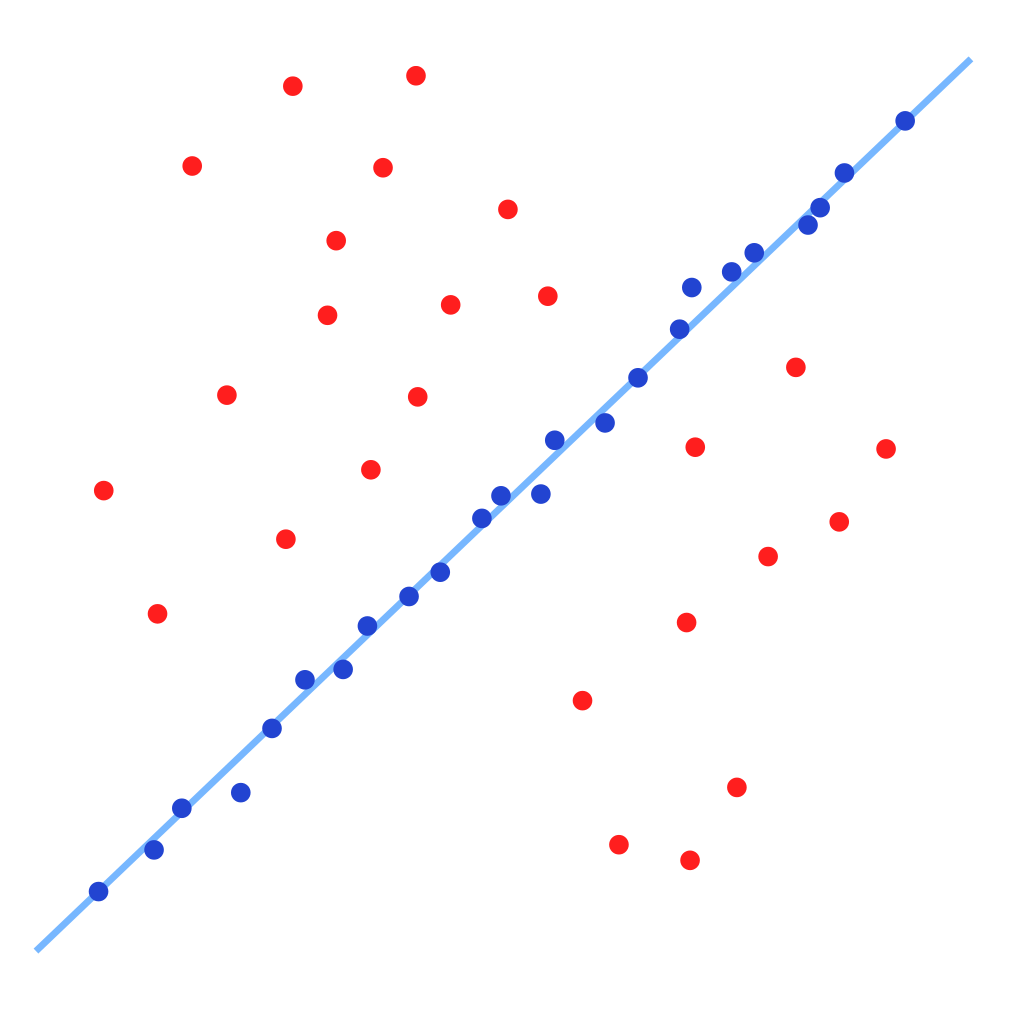
\includegraphics[width=8cm]{RANSAC.png}
\end{center}    

\subsubsection{Regressione Bayesiana}

Lo scopo della regressione bayesiana non e' di stimare puntualmente i parametri \(m, q\) ma stimarne la distribuzione.\\

Ciò ha tre  Vantaggi.\\

\begin{enumerate}
    \item Possiamo scegliere con che sicurezza (probabilita') vogliamo la stima.
    \item SI puo' avere degli intervalli di confidenza, quindi un modo oggettivo per misurare quanto la stima sia affidabile.
    \item Questo tipo di regressione parte da una distribuzione detta \textit{prior} che viene modificata dai dati.
        Questa distribuzione possiamo sceglierla per "suggerire" il comportamento che ci aspettiamo, cioè che ad esempio l'utilizzo nel tempo tenderà a salire o rimanere uguale e raramente scenderà.
    
\end{enumerate}


E' ragionevole assumere che i dati di utilizzo abbiamo un errore gaussiano additivo, quindi e' possibile rappresentare l'utilizzo del disco come:
\[u_i = r_i + \mathcal{N}(0, \sigma^2)\]

dove \(r_i\) rappresenta il reale utilizzo al istante \(i\).
\\
Questo implica che anche l'utilizzo sia rappresentabile da una distribuzione normale:
\[u_i \sim \mathcal{N}(r_i, \sigma^2)\]

Ora usando il teorema di Bayes possiamo calcolare la distribuzione dei parametri:

\[P(m | U, T) = \frac{P( U | m, T) P(m | T)}{P(U | X)}\]

dove \(P(m | U, T) \) e' la distribuzione di probabilità' del parametro \(m\) sapendo i dati di utilizzo e quelli di tempo \(U, T\).\\

e più importante e' \(P(m | T)\) e il \textit{prior} che per \textit{"""non aggiungere informazione"""} potremmo considerare uniforme ma nel nostro caso per favorire i valori di pendenza positivi e sopratutto rendere più probabili i valori piccoli rispetto ad quelli grandi poiché lo spazio occupato salirà lentamente possiamo usare un \textit{prior} esponenziale.\\\\
Questo metodo non e' applicabile direttamente su variabili continue ma possiamo approssimarlo usando un metodo MCMC nello specifico credo che il Campionamento di Gibbs sia ottimale.
\\\\
Esempio di stima bayesiana (la distribuzione a campana) vs stima puntuale (il singolo punto rappresentato dalla riga rossa tratteggiata).

\begin{center}
    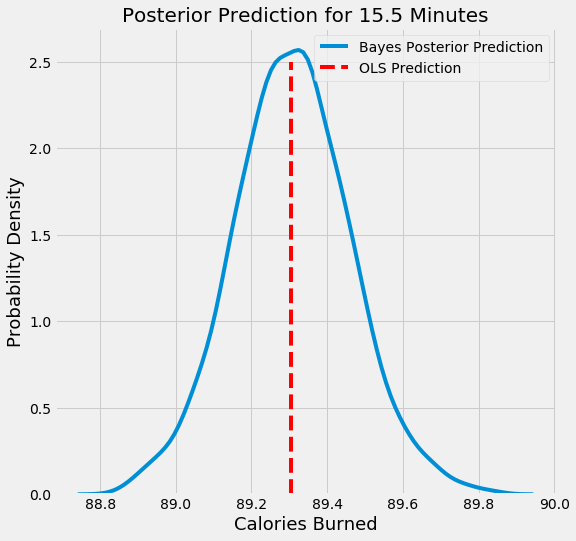
\includegraphics[width=8cm]{BvsF.png}
\end{center}

\end{document}